\documentclass[a4paper,11pt,conference]{IEEEtran}

% \usepackage[backend=biber,style=apa]{biblatex}
% \addbibresource{ref.bib}
% \usepackage{apacite}
\usepackage{url}
\usepackage{pdfpages}
\usepackage{graphicx} % For including graphics (via \includegraphics).
\usepackage{amsmath}  % Improves typographic quality of mathematical output.
\usepackage{amsfonts} % For mathematical fonts.
\usepackage{amsthm} % Needed to typeset theorem environments.
\usepackage[affil-it]{authblk} % Needed for author and affiliation.
\usepackage{amsopn} % Allows the declaration of new mathematical operators.
\usepackage{amssymb} % Extended set of mathematical symbols.
% \usepackage[left=2.5cm,right=2.5cm, top=1.5cm,bottom=1.5cm]{geometry} % Used to adjust the document margins
\usepackage{booktabs}
\usepackage{float}
\usepackage{color}
\title{\textbf{The Wing Length of Blackbirds Analysis Based on OLS Model}}
\author{35427962}
\date{\today}

\begin{document}

\maketitle

\begin{abstract}
    The purpose of this paper is to study the related factors of weight change of blackbirds. Since the weight of a blackbird varies greatly, its wing length is generally used to represent its weight instead of its real weight.

    GLM model is used to analyse information on blackbirds from the same garden in the East Midlands between 1988 and 2015. Missing values are filled in using the mean of the column data. Since the same bird is recorded many times in the dataset, it is necessary to filter the duplicate records in the data cleaning. The relevant data show that the time factor should be ignored in the research, so the earliest records of the same bird should be extracted after grouping. The classification variables are used as the independent variable and the wing length as the dependent variable for OLS fitting. As a result, the overall and single coefficients of the model are analyzed by significance. However, the goodness of fit of the model is only 44.8\%.

    The results show that there is a positive correlation between age and wing length, as well as the wing length of the male blackbirds is longer than that of the female.\\

    \noindent \textbf{Key Words:} Blackbirds; OLS; Linear Regression
  \end{abstract}

\section{Introduction}
According to Feu (n.d.) published in Mathematics Education Innovation, blackbirds have unstable body weight, sometimes less than 90g, sometimes more than 130g. They can change their weight according to conditions and gain weight on cold nights to burn approximately 5\% of their body mass for warmth. At the end of cold conditions, they lose weight and fly faster to avoid predators. The way to assess the standard size of a blackbird is to measure the length of its wings which is the distance from the carpal joint to the wingtip.

The dataset used in this analysis is 25 years of blackbirds captured in the same garden in East Midland, including foreign birds with foot rings and a small number of native British birds. When the birds are first caught, they are put on foot rings so that they can clearly trace back to the date of the first capture.

Some birds have been repeatedly trapped, according to the data requirements, this part of the data needs to be ignored. There are some missing values in the dataset, including age, gender, wing length and weight.


\section{Methods}
In this paper, NumPy, Pandas, and Statsmodels libraries in python are used to clean, calculate and analyze the dataset.

For one thing, data needs to be filled and cleaned up. Firstly, based on the information given by the dataset, vacancy value need to be filled at first. The gender of qualitative variables will be filled with the data of the same bird, while the wings and weight of quantitative variables will be filled with the average value of the whole row.

Secondly, genders and ages are recoded using dummy variables. There are only two values, namely 0 and 1. When the variables meet the conditions, the value of the matrix is 1, vice versa.

Finally, according to the suggestions in the analysis of Feu (n.d.) in the data, it can be seen that different data of the same bird species need to be ignored. I grouped the \textit{Ring Number} variable and extracted only the first observation of the grouping results, and then reconstructed the data frame to be calculated.

For another, the adjusted dataset is fitted by the ordinary least square (OLS) model. At the outset, the 0-1 matrix composed of dummy variables is used as the independent variable, while the wing length is the dependent variable. In order to prevent multicollinearity in the model, only n-1 dummy variables are selected for calculation when the type of dummy variable is n.

Therefore, the final OLS model was given as

\begin{equation}
	y = \beta_{0} + \beta_{1}x_{1} + \beta_{2}x_{2} + \beta_{3}x_{3} + \beta_{4}x_{4} + \beta_{5}x_{5} + \beta_{6}x_{6} + \epsilon
	\label{1}
\end{equation}

\noindent where $y$ is the length of blackbird's wing, $x_{1}$ is female, $x_{2}$ is male, $x_{3}$ is adult, $x_{4}$ is the first-year, and $x_{5}$ is juvenile.


\section{Results}

The following results are calculated using Statsmodels (Seabold, S. and Perktold, J., 2020) library of python as follow.

\begin{table}[!htbp]
\caption{OLS Regression Results}
% \centering
% \begin{tabular}{cccc}
\begin{tabular}{cccc}
\toprule
% Dep. Variable: & Wing & R-squared: & 0.448 \\
% Model: & OLS & Adj. R-squared: & 0.447 \\
% Method: & Least Squares & F-statistic: & 346.4 \\
% Date: & Thu, 05 Nov 2020 & Prob (F-statistic): & 3.12e-272 \\
% Time: & 00:35:47 & Log-Likelihood: & -5441.6 \\
% No. Observations: & 2141 & AIC: & 1.090e+04 \\
% Df Residuals: & 2135 & BIC: & 1.093e+04 \\
% Df Model: & 5 &  &  \\
% Covariance Type: & nonrobust
Var: & Wing & R-sq: & 0.448 \\
Model: & OLS & Ad. R-sq: & 0.447 \\
Method: & Least Squares & F: & 346.4 \\
P: & 3.12e-272 & Log-Likelihood: & -5441.6 \\
No. Obs: & 2141 & AIC: & 1.090e+04 \\
Df Res: & 2135 & BIC: & 1.093e+04 \\
Df Model: & 5 &  &  \\
Cov Type: & nonrobust \\
\bottomrule
\end{tabular}
\label{tab1}
\end{table}

\begin{table}[!htbp]
\centering
\begin{tabular}{ccccccc}
\toprule
 & coef & std err & t & P\textgreater\textbar t\textbar & [0.025 & 0.975] \\
\midrule
const & 130.45 & 0.64 & 204.07 & 0.00 & 129.20 & 131.71 \\
$Sex_{F}$ & -2.09 & 0.37 & -5.66 & 0.00 & -2.82 & -1.37 \\
$Sex_{M}$ & 2.23 & 0.36 & 6.24 & 0.00 & 1.52 & 2.93 \\
$Age_{A}$ & 1.41 & 0.54 & 2.60 & 0.01 & 0.35 & 2.47 \\
$Age_{F}$ & -2.23 & 0.54 & -4.15 & 0.00 & -3.29 & -1.18 \\
$Age_{J}$ & -3.96 & 0.57 & -6.95 & 0.00 & -5.07 & -2.84 \\
\bottomrule
\end{tabular}
\end{table}

% \begin{table}[H]
% \centering
% \begin{tabular}{cccc}
% \toprule
% Omnibus: & 9.569 & Durbin-Watson: & 1.864\\
% Prob(Omnibus): & 0.008 & Jarque-Bera (JB): & 10.200\\
% Skew: & -0.120 & Prob(JB): & 0.00610\\
% Kurtosis: & 3.238 & Cond. No. & 22.7\\
% \bottomrule
% \end{tabular}
% \end{table}

According to the table \ref{tab1}, it can be seen that the p-value of F-test of overall model is $3.12 \times 10^{-272}$, which is far less than $0.001$, and the p-value of all coefficients' T-test is less than $0.05$. This shows that the model is much significant. As well as, the value of $R^{2}$ is 0.448, which means the goodness of fit of the model was only 44.8\%, independent variables do not explain dependent variables well. The reason is that the model ignores the effect of time on wing length, which makes the model produce endogenous problems.

It can be found in the actual interpretation of the model, the wing length of female is lower than that of male significantly. Similarly, The length of wings of adult blackbirds is longer than that of juveniles. Moreover, the older the age group, the more obvious the increase of wing length.


\section{Discussion}

In this paper, the relationship between wing length and sex and age of blackbirds was quantitatively analyzed by the OLS model. The results showed that there was a positive correlation between age and wing length and males tend to have longer wings than females. The disadvantage of this paper is that it does not consider the change of time, which means that the influence of time factor on the length of blackbird wing is reflected in $\epsilon$. Since the length of blackbirds' wing has periodic time accumulation effect, the residual term must be related to its lag term, which violates the assumption of OLS estimation that the residual term is independent and identically distributed, and the result of model estimation does not conform to the excellent property of blue in Gaus-Markov theorem. In addition, the processing of the missing value is also relatively simple, there is no hierarchical interpolation fitting.


\nocite{*}

% \printbibliography
\bibliographystyle{IEEEtranN}
\bibliography{ref}

\clearpage

\section*{Appendix}

\subsection*{SAS Code}

\lstset{language=SAS}
\begin{lstlisting}
/*Load Data*/
DATA CW.violence;
LIBNAME CW 'D:\RemoteFiles\CW\Data';
INFILE 'D:\RemoteFiles\CW\Data\violence.dat';
INPUT Incident_number Month Category_of_incident Score_given_to_incident ID_of_perpetrator Sex_of_perpetrator $ Each_attack_of_perpetrator Last_attack_of_perpetrator ID_of_victim Sex_of_victim $ Each_attack_on_victim Last_attack_on_victim Victim_grade $ CRStaff;
PROC PRINT DATA=CW.violence;
RUN;

/*Question 1*/
DATA W1;
SET CW.violence (KEEP = Month Score_given_to_incident);
PROC SQL;
	CREATE TABLE CW.Q1 AS
	SELECT Month, SUM(Score_given_to_incident) as S
	FROM W1
	GROUP BY Month;
QUIT;
PROC SGPLOT;
	SERIES X = Month Y = S;
	YAXIS LABEL="Sum of Score Given to Incident";
RUN;
PROC ARIMA;
	IDENTIFY VAR=S MINIC SCAN ESACF;
RUN;
PROC ARIMA;
	IDENTIFY VAR=S;
	ESTIMATE P=0 Q=5 PLOT;
RUN;
PROC ARIMA;
	IDENTIFY VAR=S;
	ESTIMATE P=1 Q=0 PLOT;
RUN;
QUIT;

/*Question 2*/
DATA W2;
SET CW.violence (KEEP = Month Category_of_incident);
PROC SQL;
	CREATE TABLE CW.Q2 AS
	SELECT Month, Category_of_incident, COUNT(Month) AS C
	FROM W2
	GROUP BY Month, Category_of_incident
	ORDER BY Month, Category_of_incident;
QUIT;
PROC SQL;
	CREATE TABLE CW.Q2_1 AS
	SELECT Month, Category_of_incident, C, SUM(C) AS Month_C, C / SUM(C) * 100 AS Category_RATE
	FROM CW.Q2
	GROUP BY Month
	ORDER BY Month, Category_of_incident;
QUIT;
DATA CW.Q2_0;
INPUT Month Category_of_incident C Month_C Category_RATE;
CARDS;
1 2 0 0 0.0
\end{lstlisting}
\begin{lstlisting}
2 3 0 0 0.0
2 4 0 0 0.0
3 1 0 0 0.0
3 4 0 0 0.0
4 1 0 0 0.0
4 4 0 0 0.0
7 4 0 0 0.0
8 4 0 0 0.0
9 1 0 0 0.0
9 3 0 0 0.0
9 4 0 0 0.0
10 4 0 0 0.0
11 2 0 0 0.0
11 4 0 0 0.0
12 4 0 0 0.0
14 4 0 0 0.0
15 3 0 0 0.0
15 4 0 0 0.0
16 3 0 0 0.0
16 4 0 0 0.0
17 3 0 0 0.0
17 4 0 0 0.0
21 3 0 0 0.0
21 4 0 0 0.0
22 4 0 0 0.0
23 1 0 0 0.0
23 4 0 0 0.0
24 2 0 0 0.0
24 3 0 0 0.0
24 4 0 0 0.0
25 3 0 0 0.0
25 4 0 0 0.0
26 3 0 0 0.0
26 4 0 0 0.0
27 3 0 0 0.0
28 2 0 0 0.0
28 4 0 0 0.0
29 2 0 0 0.0
29 4 0 0 0.0
30 3 0 0 0.0
30 4 0 0 0.0
;
RUN;

/*Optian a*/
DATA CW.Q2_2;
	SET CW.Q2_0 CW.Q2_1;
RUN;
PROC SORT DATA=CW.Q2_2;
	BY MONTH Category_of_incident;
RUN;
PROC SGPLOT DATA=CW.Q2_2;
	SERIES X = Month Y = Category_RATE / GROUP = Category_of_incident;
	YAXIS LABEL="The Rate of Attacks in Each Category (%)";
	TITLE '';
RUN;
DATA CW.Q2_2_near_miss;
	SET CW.Q2_2 (KEEP = Month Category_of_incident Category_RATE);
	WHERE  Category_of_incident = 1;
RUN;
PROC SGPLOT DATA=CW.Q2_2_near_miss;
	SERIES X = Month Y = Category_RATE;
\end{lstlisting}
\begin{lstlisting}
	TITLE '';
	YAXIS LABEL="The Percentage of Near Miss (%)";
RUN;

DATA CW.Q2_2_assault;
	SET CW.Q2_2 (KEEP = Month Category_of_incident Category_RATE);
	WHERE  Category_of_incident = 2;
RUN;
PROC SGPLOT DATA=CW.Q2_2_assault;
	SERIES X = Month Y = Category_RATE;
	TITLE '';
	YAXIS LABEL='The Percentage of Assault (%)';
RUN;
DATA W2_1;
	SET CW.violence (KEEP = Month Category_of_incident);
PROC SQL;
	CREATE TABLE W2_Total AS
	SELECT Month, COUNT(Month) AS C
	FROM W2_1
	GROUP BY Month
	ORDER BY Month;
QUIT;
PROC SQL;
	CREATE TABLE W2_Assault AS
	SELECT Month, COUNT(Month) AS A
	FROM W2_1
	WHERE Category_of_incident = 2
	GROUP BY Month
	ORDER BY Month;
QUIT;
DATA Q2_Merged;
	MERGE W2_Total W2_Assault;
	BY Month;
	RETAIN Assault;
	IF A = . THEN Assault = 0;
	ELSE Assault = A;
PROC CORR DATA=Q2_Merged ;
	VAR C Assault;
RUN;

/*Optian (b)*/
DATA CW.Q2_3;
	SET CW.Q2_1;
	WHERE Month > 15;
	Category = PUT(Category_of_incident, 2.);
	DROP Category_of_incident;
PROC GCHART DATA=CW.Q2_3;
	PIE Category /
	VALUE=NONE
	PERCENT=ARROW
	SLICE=ARROW
	NOHEADING;
	TITLE '';
RUN;
QUIT;

/*Question 3*/
DATA CW.Q3;
	SET CW.violence (KEEP = Category_of_incident Score_given_to_incident Sex_of_perpetrator);
PROC ANOVA DATA=CW.Q3;
	CLASS Sex_of_perpetrator Category_of_incident;
\end{lstlisting}
\begin{lstlisting}
	MODEL Score_given_to_incident=Sex_of_perpetrator Category_of_incident Sex_of_perpetrator*Category_of_incident;
	MEANS Sex_of_perpetrator Category_of_incident Sex_of_perpetrator*Category_of_incident/DUNCAN;
RUN;
PROC SQL;
	CREATE TABLE CW.Q3_1 AS
	SELECT Sex_of_perpetrator, Category_of_incident, SUM(Each_attack_of_perpetrator) AS Each_SUM
	FROM CW.violence
	GROUP BY Category_of_incident, Sex_of_perpetrator
	ORDER BY Category_of_incident, Sex_of_perpetrator;
QUIT;
PROC GCHART DATA=CW.Q3_1;
	VBAR Sex_of_perpetrator /SUMVAR=Each_SUM GROUP=Category_of_incident;
	TITLE 'Score Given to Incident by Sex';
RUN;

/*Question 4*/
DATA CW.Q4;
	SET CW.violence (KEEP=Month Victim_grade);
	WHERE Victim_grade = "SN" OR Victim_grade = "CR";
PROC FREQ DATA=CW.Q4;
	TABLES Month * Victim_grade /OUT=W4_FREQ OUTPERCENT;
RUN;
PROC PRINT DATA=W4_FREQ;
RUN;
DATA W4_FREQ_1;
	SET W4_FREQ (KEEP=Month Victim_grade PCT_ROW);
	PCT_ROW = PCT_ROW;
DATA W4_FREQ_0;
INPUT Month Victim_grade $ PCT_ROW;
CARDS;
1 CR 0.00000
2 CR 0.00000
3 CR 0.00000
4 CR 0.00000
5 CR 0.00000
6 CR 0.00000
7 CR 0.00000
8 CR 0.00000
9 CR 0.00000
11 CR 0.00000
16 CR 0.00000
17 SN 0.00000
24 SN 0.00000
28 SN 0.00000
29 SN 0.00000
30 SN 0.00000
;
DATA CW.Q4_FREQ;
	SET W4_FREQ_1 W4_FREQ_0;
PROC SORT DATA=CW.Q4_FREQ;
	BY Month Victim_grade;
RUN;
PROC SGPLOT DATA=CW.Q4_FREQ;
	SERIES X = Month Y = PCT_ROW/GROUP=Victim_grade;
	TITLE 'Relative Frequencies of Victim Grade';
	YAXIS LABEL='Relative Frequencies';
RUN;

/*Question 5*/
\end{lstlisting}
\begin{lstlisting}
DATA CW.Q5;
	SET CW.violence (KEEP=ID_of_victim);
	ID = PUT(ID_of_victim, 2.);
	DROP ID_of_victim;
RUN;
PROC FREQ DATA=CW.Q5;
	TABLES ID/OUT=CW.Q5_FREQ;
RUN;
PROC GCHART DATA=CW.Q5;
	PIE ID /
	VALUE=NONE
	PERCENT=ARROW
	SLICE=ARROW
	NOHEADING
	OTHER=0;
	TITLE 'Frequency of Particular Individuals Attacked';
RUN;
QUIT;

/*Question 6*/
/*number*/
DATA CW.Q6_Number;
	SET CW.violence (KEEP=Each_attack_of_perpetrator Last_attack_of_perpetrator CRStaff);
	WHERE Last_attack_of_perpetrator = 1;
PROC GENMOD DATA=CW.Q6_Number PLOTS=ALL;
	MODEL Each_attack_of_perpetrator = CRStaff / DIST=POSSION LINK = LOG;
	OUTPUT OUT=bclassg_Number p=pred_Number;
RUN;
/*severity of the attacks*/
DATA CW.Q6_Severity;
	SET CW.violence (KEEP=Category_of_incident Score_given_to_incident Each_attack_of_perpetrator CRStaff);
PROC LOGISTIC PLOTS=ALL;
	MODEL Score_given_to_incident=CRStaff;
	OUTPUT OUT=bclassg_Severity p=pred_Severity;
RUN;
QUIT;
\end{lstlisting}


\clearpage

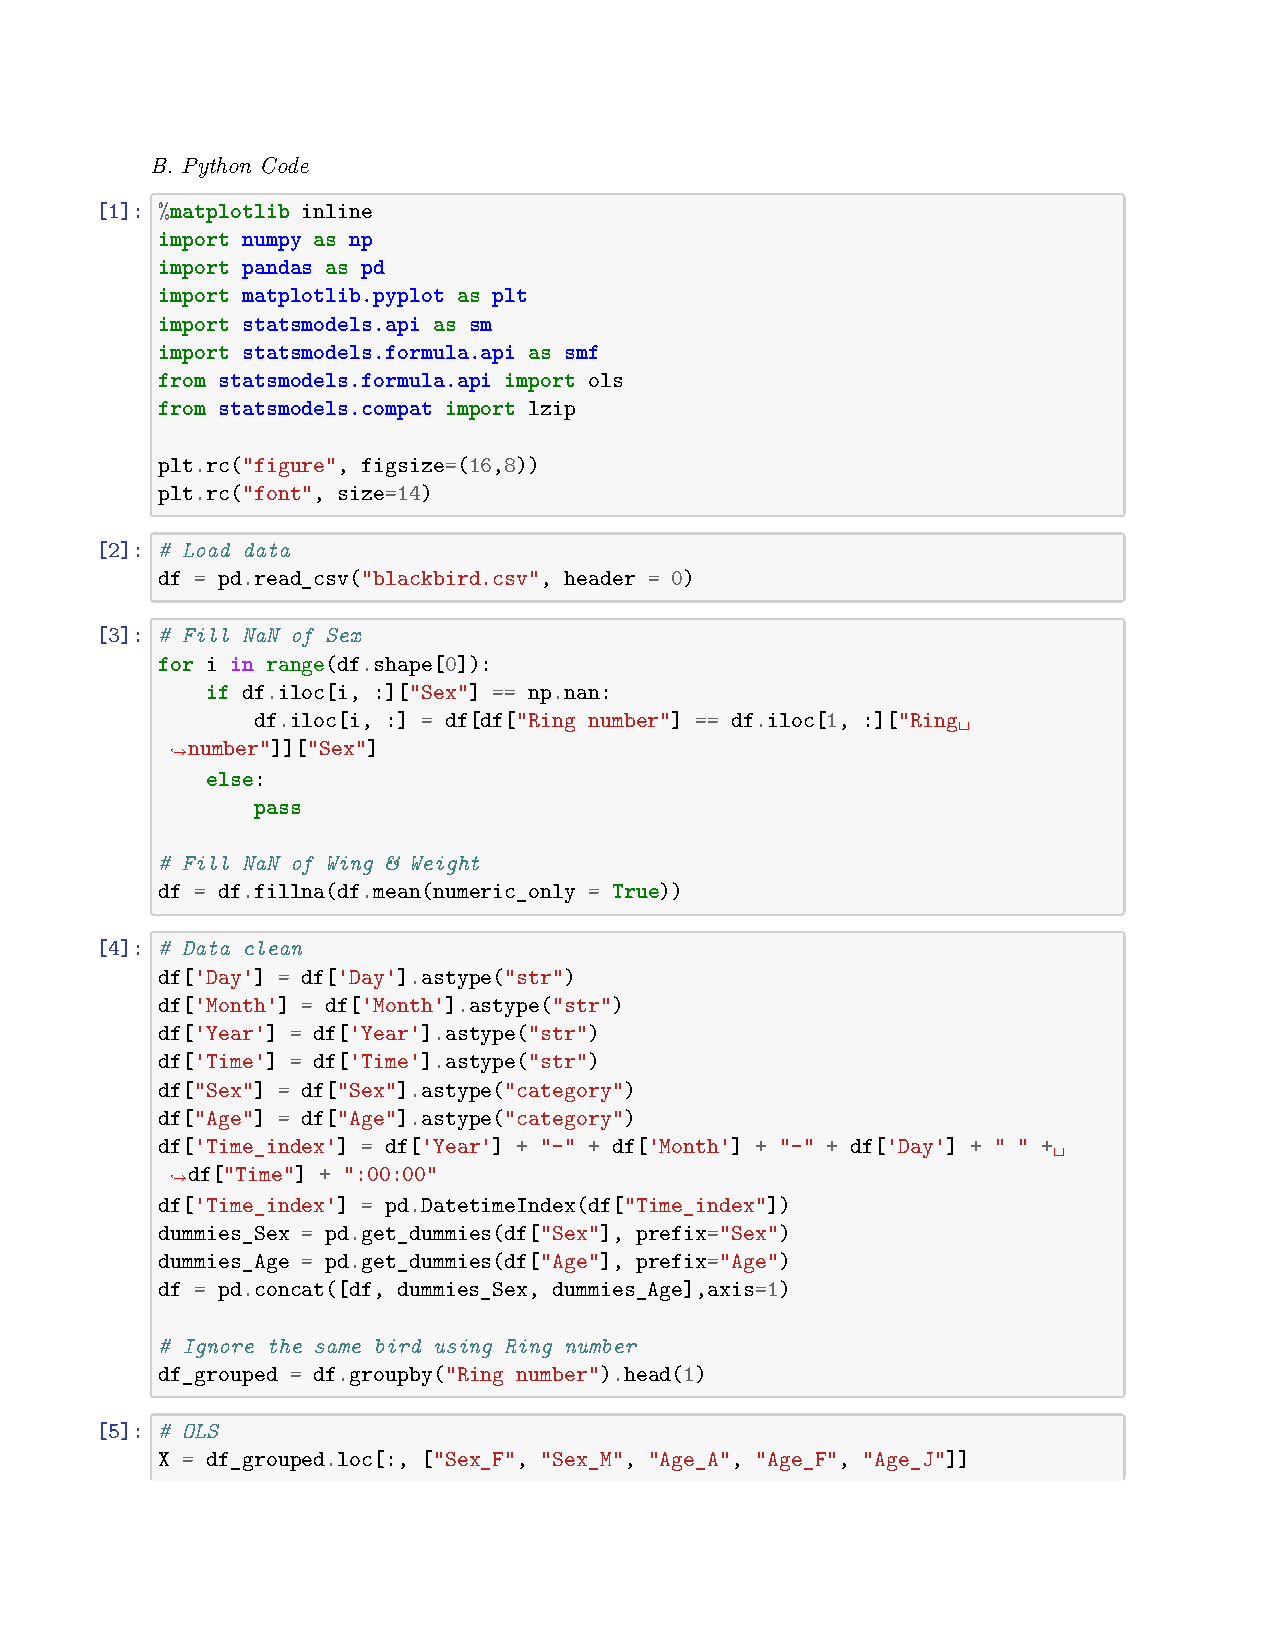
\includepdf[pages={1-5}]{Code/Code.pdf} 

\end{document}
